\chapter{General Analysis Strategy}
\label{chap:AnaStrategy}
\section{General R-Parity Conserving SUSY Search Strategy}
\indent In most R-parity conserving SUSY searches, the sought after super-symmetric particle will mostly be produced in pairs.  Each particle decays via a chain that ends in a stable, weakly interacting lightest super-symmetric particle (LSP).  Because the LSP is weakly interacting, it will not be directly detectable by the ATLAS detector and must be inferred via momentum conservation as \MET.  The rest of the products from the decay chain will be a series of standard model particles which can also be a combination of visible particles and invisible neutrinos.  ~\\
\indent All searches must distinguish between true SUSY processes and standard model physics processes that mimic the decay products of the target SUSY process.  Traditional search methods often place special emphasis on identifying the LSP as this is the one part that is unique to the SUSY events.  Practically this means searching for events with large amount of \MET.  The decay of the original SUSY particle generates large amounts of momenta for the LSP in regions with a large mass splitting between the original SUSY particle and LSP.  Traditional searches therefore target the large amount of \MET generated by the LSP can be used to identify SUSY events and is sensitive to regions where the SUSY particle and LSP decay products have large mass splittings. ~\\
\section{General Strategies in Compressed Regions}
\indent When mass splitting between the original SUSY particle and its decay products become small, there is little energy left over to generate momenta in those decay products.  The result is a LSP with little momenta.  The traditional strategy of searching for events with large amount of \MET therefore fails in this region of parameter space.  Any region where the decay products of the target particle have little momenta is considered a compress region.  ~\\
\indent  For our specific analysis, the super-partner of the top, the s-top (\stop) is expected to decay into a neutralino and top.  When the \stop~mass is close to that of the top mass plus the neutralino mass, both the top and neutralino gain very little momenta from the decay.  The invisible neutralinos in turn generate very little missing transverse energy.  This leaves only the visible tops which are mimicked by standard model ttbar.  The same problem arises in many other searches if the mass splittings are small or at a particular value where the decay products gains very little momenta.  However, the soft decay products can gain additional momenta if the entire system is boosted by strong initial state radiation (ISR). \\
\indent The true goal of the searches have always been to identify the presence of the LSPs and use their presence to distinguish the target events from SM processes.  Instead of targeting events with large amount of \MET, we use the correlations between the LSP momenta and any ISR jets to identify LSPs in compressed regions.  It is precisely because most of the momenta of the decay products are not coming from the decays but from the boost via strong ISR that the correlation between decay products and ISR tends to be extremely strong.  In this way, we turn an experimental difficulty into a strength.  \\
\indent The relationship between the decay products and ISR also has an additional benefit of being model independent.  This correlation is dictated solely by relativistic kinematics rather than the underlying QFT of any particular model.  Essentially because the decay products gain little energy from the decay, the majority of the decay product's energy is coming from the kick of the ISR.  Therefore, the direction and magnitude of the momenta of the decay products are determined mostly by two things, how heavy the decay products are and how hard they are kicked by the ISR. For the $p p \rightarrow \antibar{\stop} \rightarrow t\ninoone\tbar\ninoone$ process, the relationship is given by equation \ref{eqn:theory_MET_ISR}. This ratio between the invisible decay products and the total ISR pt is called \RISR. \\

%\begin{equation}
\begin{align}
\MET \equiv p_{\ninoone\ninoone,~T}^{~\mathrm{lab}} \sim \gamma_{\stop\stop}^{~\mathrm{lab}} \beta_{\stop\stop}^{~\mathrm{lab}} E_{\ninoone\ninoone}^{~\stop\stop} 
\sim \frac{\PTISR}{m_{\stop\stop}} 2\gamma_{\stop}^{\stop\stop} m_{\tilde{\chi}} \sim
\PTISR \frac{ 2\gamma_{\stop}^{\stop\stop} m_{\tilde{\chi}} }{ 2\gamma_{\stop}^{\stop\stop} m_{\stop} } \sim
\PTISR \frac{m_{\ninoone}}{m_{\stop}}\implies\\
\RISR \equiv \frac{\MET}{\PTISR} \sim \frac{m_{\ninoone}}{m_{\stop}}~,\quad\quad\quad\quad\quad\quad\quad\quad\quad\quad\quad\quad
\label{eqn:theory_MET_ISR}
\end{align}
%\end{equation}
\indent Figure \ref{fig:stop_400_227_ISR_MET_truth} shows the correlations between the di-neutralino system, decay products of the \antibar{\stop}~system, and the ISR system before taking into account detector resolution effects. As you can see, the correlation between the ISR pt and the \MET follows a straight line with a slope that is predicted by equation \ref{eqn:theory_MET_ISR}. \\

\indent Notice that although the \MET is directly proportional to the combined di-LSP pt, the ratio between \MET and ISR pt is still proportional to the mass of a single LSP and original sparticle.  This means that the back to back boost between the two original sparticles in this case the two \stop~ do not affect the correlation between the observable \MET and ISR pt.  Only the di-LSP pt is measurable because the LSPs are invisible and cannot be measured alone.  Although the LSP's can individually gain momenta from the back to back boost of the sparticles against one another, the back to back momenta will exactly cancel resulting in zero measurable \MET for the di-LSP system regardless of the back to back boost of the two sparticles.  The di-LSP system only gains pt by inheriting it from the boost of di-sparticle system by the ISR system.  The fraction of the momenta that is inherited by the di-LSP system 
from the pt of the di-sparticle system is exactly $\frac{m_{LSP}}{m_{sparticle}}$ if the sparticle decay gives no additional momenta to the LSP.  Because the di-sparticle pt must be equal and opposite that of the ISR pt by momenta conservation, the ratio between observable \MET and ISR pt or \RISR is given by \ref{eqn:theory_MET_ISR}.  Figure \ref{ig:stop_400_227_ISR_MET_truth} shows the correlation between the \MET and ISR pt in simulation for the $p p \rightarrow \antibar{\stop} \rightarrow t\ninoone\tbar\ninoone$ process for the case when the sparticle (\stop) has mass 400 GeV and the LSP (\ninoone) has mass 227 GeV and the top has mass 172.5 GeV. The preferred ratio between the \met and ISR pt is shown by a line with the slope that is exactly predicted by equation \ref{eqn:theory_MET_ISR}.  Generating an offshell top far from the kinematic limit of $m_{\stop}$ minus $m_{\ninoone}$ can free up additional energy that can boost the LSP and spoil this correlation but the probability of this deviation is limited by the top width of ~1.3 GeV.  ~\\

\begin{figure}[h!]
  \centering
	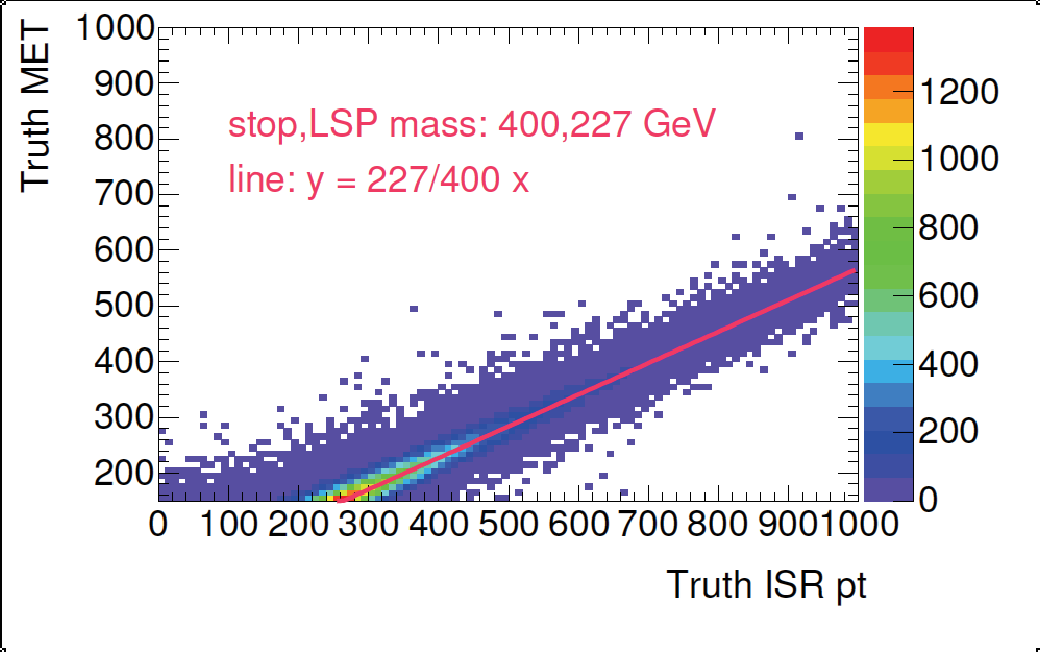
\includegraphics[width=0.65\textwidth]{./figures/MET_ISR.png}
\caption{\label{fig:stop_400_227_ISR_MET_truth}{Distribution of di-neutralino pt, as represented by \met, vs total ISR pt before factoring in detector resolution for (400,227) \stop,\ninoone~mass point.  The preferred ratio between the \met and ISR pt can be predicted using special relativity kinematics by equation \ref{eqn:theory_MET_ISR}.  Deviation from this ratio is limited by the top width. }}
\end{figure}

\indent By constructing variables that capitalize on this correlation we are able to separate signal from standard model backgrounds which do not peak sharply in the \RISR variable.  On a practical note, the increase in center-of-mass energy from 8 to 13 TeV can mean up to an order of magnitude higher probability of emitting strong ISR.  The 13 TeV dataset presents a golden opportunity to search for many new physics processes that need a boost from strong ISR in order to be detected. \\